\section{Objets DICOM}

\frame
{
 	\frametitle{Information Object Definition}
  	L'IOD d\'efinit, pour un IO sp\'ecifique, quelles sont les attributs qu'on doit/peut trouver dans l'objet.
  	\begin{description}
    		\item[Normalized IOD]~\\
			Repr\'esente une entit\'e unique du monde r\'eel (patient, visite, examen, r\'esultat, interpr\'etation,\ldots).
			Complexe et peu performant.
    		\item[Composite IOD]~\\
			Repr\'esente certains d\'etails de plusieurs objets du monde r\'eel et les relations entre ces objets (nom du patient, date de l'examen,\ldots)
		\item[Attributes]~\\
			Les attributs d'un IOD sont les propri\'et\'es d'un \'el\'ement du monde r\'eel.
  	\end{description}
}

\frame
{
 	\frametitle{IOD composite}
 	\begin{itemize}
		\item IOD : agr\'egat d'\emph{Information Entities} ou \emph{IE}.
   		\item Une IE contient un ou plusieurs \emph{Modules}.
		\begin{description}
			\item[Mandatory] Module obligatoire.
			\item[Conditional] Module conditionnel (obligatoire selon certaines conditions).
			\item[User Option] Module optionnel.
		\end{description}
   		\item Les modules sont compos\'es d'\emph{Attributs} (= valeurs).
		\begin{description}
			\item[1] Obligatoire.
			\item[2] Obligatoire - peut \^etre vide.
			\item[3] Optionnel.
			\item[<1/2>C] Conditionnel.
		\end{description}
 	\end{itemize}

	\begin{alertblock}{En pratique}
		Un objet DICOM est presque toujours une instance d'un IOD composite.
	\end{alertblock}
}

\frame
{
 	\frametitle{IOD composite}
	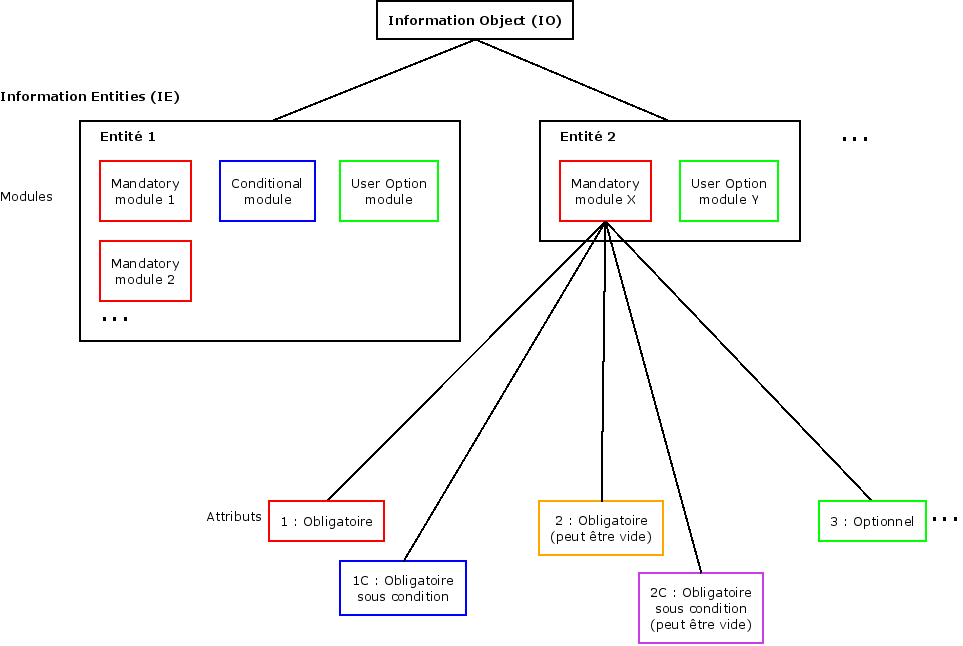
\includegraphics[width=\linewidth]{./figures/IO-composite.png}
}
\frame
{
	\frametitle{Exemple d'IOD : image CR}
	
	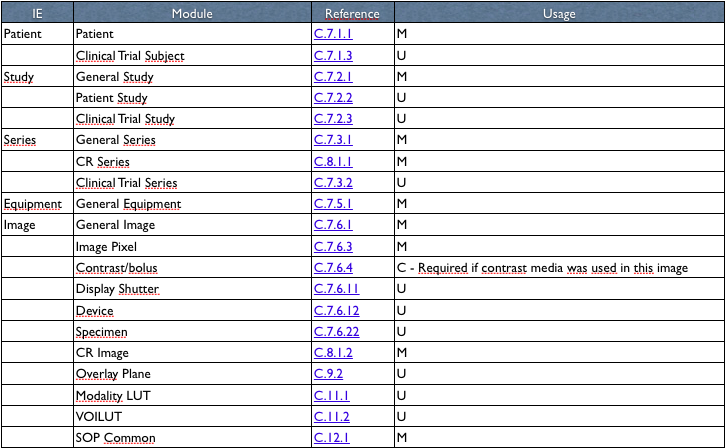
\includegraphics[width=\linewidth]{./figures/IOD-exemple.png}
}

\frame
{
	\frametitle{Sch\'ema de l'IOD image CR}
	\label{imageCR-IOD}
	
	\begin{center}
		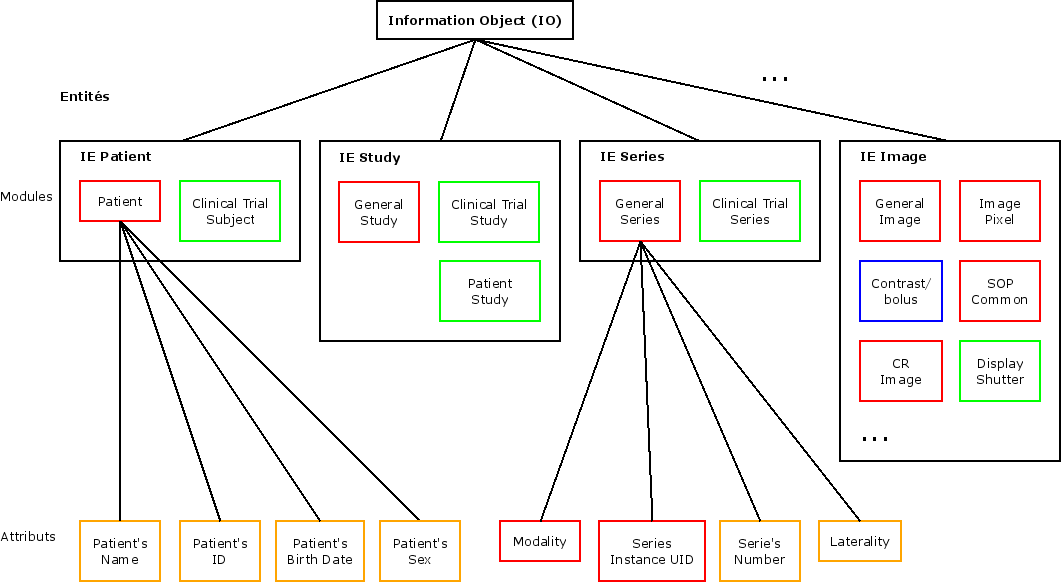
\includegraphics[width=\linewidth]{./figures/IO-definition.png}
	\end{center}
}

\frame
{
	\frametitle{Objet}
	\begin{itemize}
		\item Terminologie : objet = Data Set (\emph{e.g.} ensemble de donn\'ees).
		\item Un Data Set contient des Data Elements.
		\item Chaque Data Element donne une valeur \`a un et un seul attribut de l'IOD.
		\item Contenu d'un Data Element :
		\begin{itemize}
			\item �tiquette d'identification (\emph{Tag}) contenant deux num\'eros.
			\item Type (\emph{VR} = \emph{Value Representation}).
			\item Taille en m\'emoire de la valeur.
			\item Valeur.
		\end{itemize}
	\end{itemize}
}

\frame
{
	\frametitle{Objet}
	
	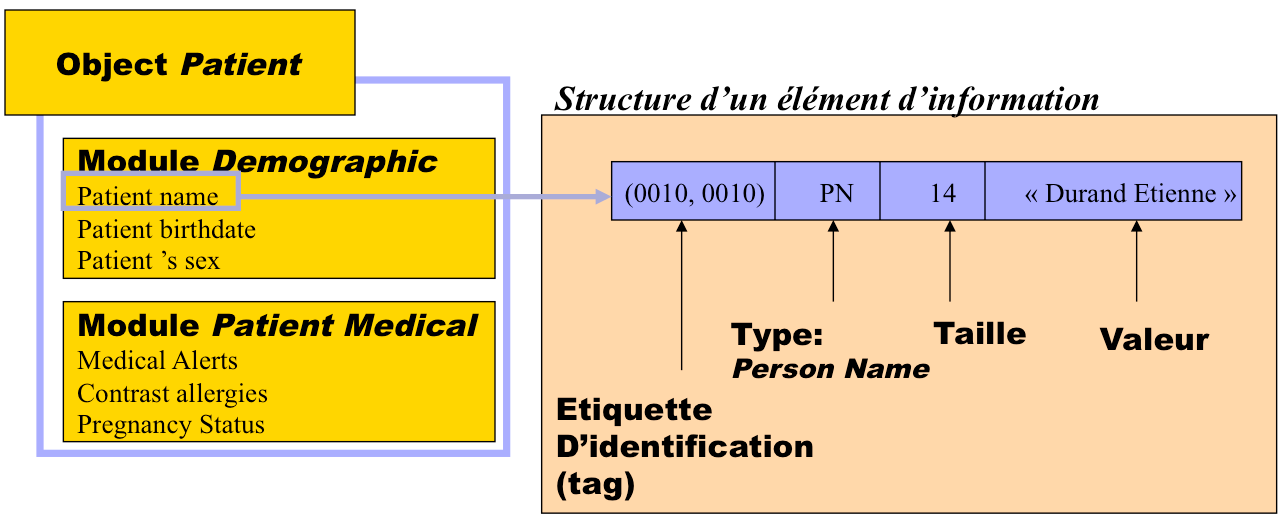
\includegraphics[width=\linewidth]{./figures/objet-dicom.png}
}

\frame
{
	\frametitle{Exemple d'objet : Examen (\emph{Study})}
	
	\begin{center}
		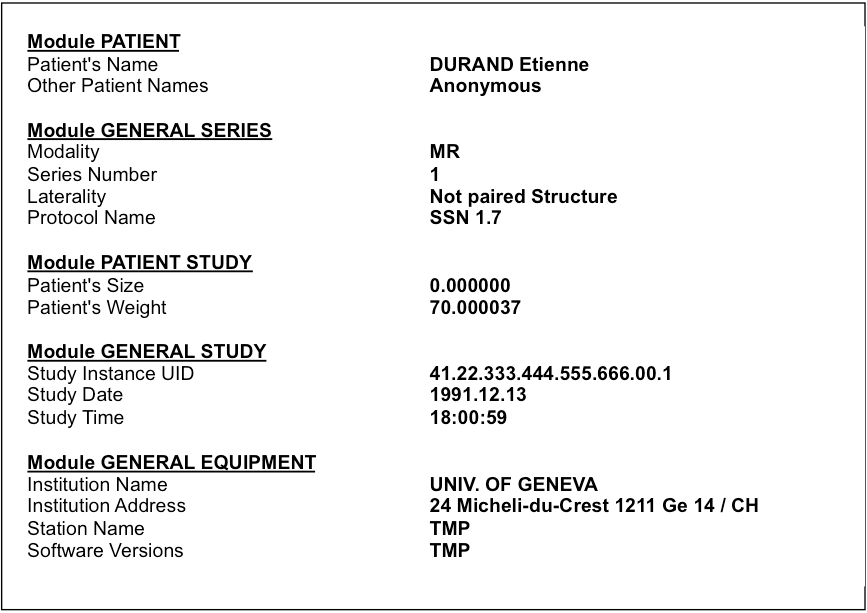
\includegraphics[width=.9\linewidth]{./figures/examen.png}
	\end{center}
}

\frame
{
	\frametitle{Exemple d'objet : Image IRM}
	
	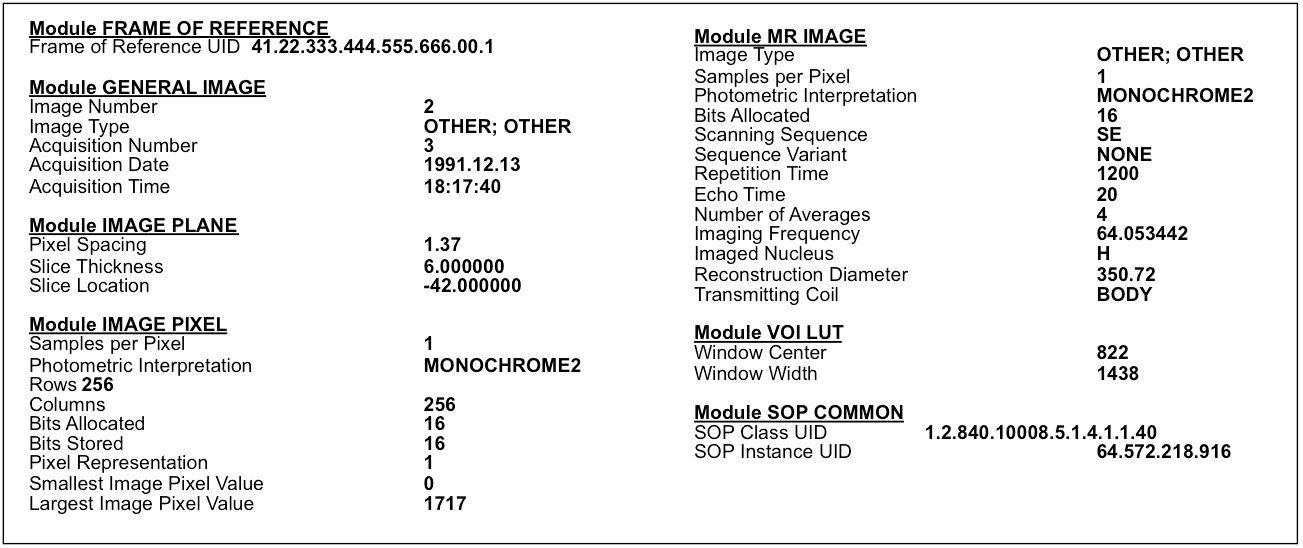
\includegraphics[width=\linewidth]{./figures/irm.png}
}

\frame
{
	\frametitle{Fichier DICOM}
	
	\begin{itemize}
		\item Agr\'eger l'ensemble des objets dans un fichier.
		\begin{itemize}
			\item Ent\^ete : pr\'e-ent\^ete et objets.
			\item Image : donn\'ees brutes de l'image.
		\end{itemize}
		\item Les d\'etails au prochain cours.
	\end{itemize}
}

